%----------------------------------------------------------------------------------------
%    PACKAGES AND THEMES
%----------------------------------------------------------------------------------------

\documentclass[aspectratio=169,xcolor=dvipsnames]{beamer}
\usetheme{SimpleDarkBlue}

\usepackage{hyperref}
\usepackage{graphicx} % Allows including images
\usepackage{booktabs} % Allows the use of \toprule, \midrule and \bottomrule in tables
\usepackage{tikz} % For diagrams
\usepackage{fontawesome} % For icons

%----------------------------------------------------------------------------------------
%    TITLE PAGE
%----------------------------------------------------------------------------------------

\title{Interactive Multimodal GPT System}
\subtitle{Progress Report}

\author{Haowei Gao}

\institute
{
    Department of Bioengineering
}
\date{July 28, 2025}

%----------------------------------------------------------------------------------------
%    PRESENTATION SLIDES
%----------------------------------------------------------------------------------------

\begin{document}

\begin{frame}
    % Print the title page as the first slide
    \titlepage
\end{frame}

\begin{frame}{Overview}
    % Throughout your presentation, if you choose to use \section{} and \subsection{} commands, these will automatically be printed on this slide as an overview of your presentation
    \tableofcontents
\end{frame}

%------------------------------------------------
\section{Core Features \& Workflow}
%------------------------------------------------

\begin{frame}{Core Capabilities}
    \begin{columns}[c]
        \column{.5\textwidth}
        \textbf{Key Features}
        \begin{itemize}
            \item \textbf{Multimodal Analysis}: Tactile + Vision + Text
            \item \textbf{Interactive Web UI}: React-based with drag-and-drop
            \item \textbf{AI-Powered Reasoning}: GPT integration via Together AI
            \item \textbf{Prompt Engineering}: Automated optimization strategies
        \end{itemize}

        \column{.45\textwidth}
        \textbf{Supported Modalities}
        \begin{enumerate}
            \item \textbf{Tactile-Text}: Sensor data + descriptions
            \item \textbf{Vision-Text}: Images + text analysis
            \item \textbf{Tactile-Vision-Text}: Complete multimodal fusion
            \item \textbf{Text Only}: Pure text processing
        \end{enumerate}
    \end{columns}
\end{frame}

%------------------------------------------------

    \begin{frame}{Workflow Process}
        \begin{center}
            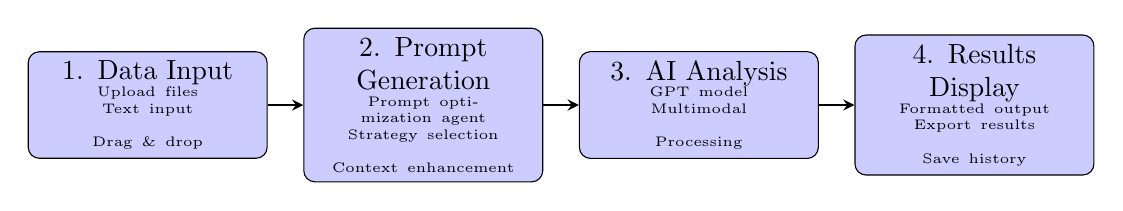
\begin{tikzpicture}[node distance=3.5cm]
                \tikzstyle{process} = [rectangle, draw, fill=blue!20, text width=2.8cm, text centered, rounded corners, minimum height=1.2cm]
                \tikzstyle{arrow} = [thick,->,>=stealth]
                
                \node (input) [process] {1. Data Input\\\tiny{Upload files\\Text input\\Drag \& drop}};
                \node (prompt) [process, right of=input] {2. Prompt Generation\\\tiny{Prompt optimization agent\\Strategy selection\\Context enhancement}};
                \node (analysis) [process, right of=prompt] {3. AI Analysis\\\tiny{GPT model\\Multimodal\\Processing}};
                \node (output) [process, right of=analysis] {4. Results Display\\\tiny{Formatted output\\Export results\\Save history}};
                
                \draw [arrow] (input) -- (prompt);
                \draw [arrow] (prompt) -- (analysis);
                \draw [arrow] (analysis) -- (output);
            \end{tikzpicture}
        \end{center}
        
        \vspace{1.2cm}
        \begin{block}{Process Flow}
            The system processes multimodal data through four main stages: data input, intelligent prompt generation, AI-powered analysis, and comprehensive result presentation.
        \end{block}
    \end{frame}

%------------------------------------------------
\section{Recent Literature Highlight}
%------------------------------------------------

\begin{frame}{Prompt Engineering Studies}
    \begin{block}{Recent Advances in Prompt Engineering}
        \begin{itemize}
            \item \textbf{Analogical Prompting} (Yasunaga et al., ICLR 2024) — prompts the LLM to self-generate relevant exemplars (and optional tutorials) before answering; consistently beats 0-shot / few-shot chain-of-thought on GSM8K, MATH and Codeforces (+≈4\% accuracy).
            
            \item \textbf{Comprehensive Survey of Prompt Engineering} (Liu et al., 2024) — organises zero/one/multi-shot, role, CoT, self-consistency and retrieval-augmented prompting into a single taxonomy and introduces robustness metrics for evaluating prompt methods.
            
            \item \textbf{Practical Prompting Guide} (Anthropic, 2023) — field-tested rules ("be explicit, give examples, ask for chain-of-thought, set model role") that cut hallucinations and raise internal QA accuracy by ≈38\%.
        \end{itemize}
    \end{block}
    
    \vspace{0.3cm}
    \begin{center}
        \small{These studies inform our prompt optimization strategies and guide the development of more effective multimodal reasoning approaches.}
    \end{center}
\end{frame}

%------------------------------------------------
\section{Technical Architecture}
%------------------------------------------------

\begin{frame}{System Architecture}
    \begin{center}
        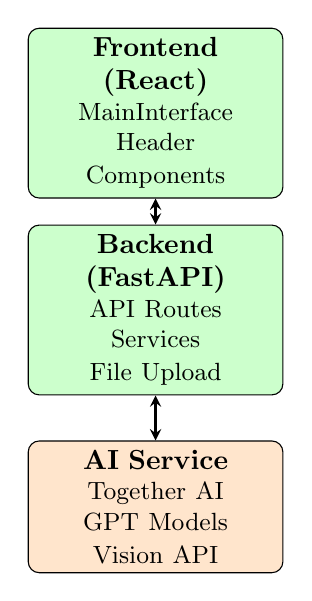
\begin{tikzpicture}[node distance=2.5cm]
            \tikzstyle{layer} = [rectangle, draw, fill=green!20, text width=3cm, text centered, rounded corners, minimum height=1.5cm]
            \tikzstyle{service} = [rectangle, draw, fill=orange!20, text width=3cm, text centered, rounded corners, minimum height=1.5cm]
            \tikzstyle{arrow} = [thick,<->,>=stealth]
            
            \node (frontend) [layer] {\textbf{Frontend (React)}\\\small{MainInterface\\Header\\Components}};
            \node (backend) [layer, below of=frontend] {\textbf{Backend (FastAPI)}\\\small{API Routes\\Services\\File Upload}};
            \node (ai) [service, below of=backend] {\textbf{AI Service}\\\small{Together AI\\GPT Models\\Vision API}};
            
            \draw [arrow] (frontend) -- (backend);
            \draw [arrow] (backend) -- (ai);
        \end{tikzpicture}
    \end{center}
\end{frame}

%------------------------------------------------

    \begin{frame}{Code Structure}
        \begin{columns}[c]
            \column{.45\textwidth}
            \vspace{-0.5cm}
            \begin{center}
                \includegraphics[width=0.9\textwidth]{code structure.png}
            \end{center}

            \column{.5\textwidth}
            \textbf{Backend Structure}
            \begin{itemize}
                \item \texttt{main.py} - FastAPI app, CORS, routers
                \item \texttt{services/} - Core business logic
                \begin{itemize}
                    \item \texttt{gpt\_integration.py} - Together AI API
                    \item \texttt{prompt\_engineering.py} - Prompt optimization
                \end{itemize}
            \end{itemize}
            
            \textbf{Frontend Structure}
            \begin{itemize}
                \item \texttt{frontend/src/} - React application
                \begin{itemize}
                    \item \texttt{MainInterface.js} - Main dashboard
                    \item \texttt{Header.js} - Navigation header
                    \item \texttt{components/} - UI components
                \end{itemize}
            \end{itemize}
        \end{columns}
    \end{frame}

%------------------------------------------------
\section{Implementation Status \& Roadmap}
%------------------------------------------------

\begin{frame}{Implemented Features}
    \begin{columns}[c]
        \column{.5\textwidth}
        \textbf{Completed Features}
        \begin{itemize}
            \item \textbf{Web Interface}: React-based dashboard with modern UI
            \item \textbf{File Upload System}: Support for image and text files
            \item \textbf{Multimodal Analysis}: Vision-text and text-only modes
            \item \textbf{API Integration}: Together AI with Llama-Vision-Free model
            \item \textbf{Real-time Feedback}: Live status updates and notifications
        \end{itemize}

        \column{.45\textwidth}
        \textbf{In Progress / Limitations}
        \begin{itemize}
            \item \textbf{Tactile Data Processing}: File upload available but not yet processed
            \item \textbf{Prompt Optimization}: Currently simulated (not AI-driven)
            \item \textbf{Advanced Templates}: Basic prompt templates implemented
            \item \textbf{History Management}: Session-based only (no persistence)
        \end{itemize}
    \end{columns}
    
    \vspace{0.5cm}
    \begin{block}{Current Status}
        Core web interface and vision-text analysis are fully functional. Tactile data processing and AI-driven prompt optimization are planned for next phase.
    \end{block}
\end{frame}



\begin{frame}{Project Summary}
    \begin{columns}[c]
        \column{.5\textwidth}
        \textbf{Research Contribution}
        \begin{itemize}
            \item \textbf{Multimodal Reasoning}: Tactile-text-vision integration using GPT models
            \item \textbf{Prompt Engineering}: Advanced techniques based on latest literature
            \item \textbf{Interactive System}: Real-time multimodal data processing
            \item \textbf{Modern Architecture}: FastAPI + React with Together AI integration
        \end{itemize}

        \column{.45\textwidth}
        \textbf{Technical Innovation}
        \begin{itemize}
            \item \textbf{Unified Analysis}: Single endpoint for multiple modality combinations
            \item \textbf{Simulated Optimization}: AI prompt enhancement framework
            \item \textbf{Dynamic UI}: Context-aware file upload and processing
            \item \textbf{Extensible Design}: Modular services for future enhancements
        \end{itemize}
    \end{columns}
    
    \vspace{0.3cm}
    \begin{block}{Current Status \& Next Steps}
        \small
        \textbf{Completed}: Web interface, vision-text analysis, file management system \\
        \textbf{In Progress}: Tactile data processing, AI-driven prompt optimization \\
        \textbf{Future Work}: Advanced multimodal fusion, persistent history, batch processing
    \end{block}
\end{frame}

%------------------------------------------------

\begin{frame}
    \Huge{\centerline{\textbf{Thank You!}}}
    \vspace{0.5cm}
    \begin{block}{References}
        \small
        \begin{itemize}
            \item Yasunaga, M., Chen, X., Li, Y., Pasupat, P., Leskovec, J., Liang, P., ... \& Zhou, D. (2023). Large language models as analogical reasoners. \textit{arXiv preprint arXiv:2310.01714}.
            
            \item Sahoo, P., Singh, A. K., Saha, S., Jain, V., Mondal, S., \& Chadha, A. (2024). A systematic survey of prompt engineering in large language models: Techniques and applications. \textit{arXiv preprint arXiv:2402.07927}.
            
            \item Anthropic. (2023). A Practical Guide to Prompt Engineering. \textit{Anthropic Technical Report}.
        \end{itemize}
    \end{block}
\end{frame}

%----------------------------------------------------------------------------------------

\end{document} 